\chapter{Applicazione desktop}
\label{Cha:desktop}
\thispagestyle{empty}

Il capitolo seguente sarà incentrato sulla presentazione dell'applicazione desktop e delle sue interfacce e funzionalità.

\section{Sviluppo}
L'applicazione è stata creata su \textit{Visual Studio}, utilizzando il framework \textit{WPF} (Windows Presentation Foundation) che fornisce agli sviluppatori un modello di programmazione unificato per la creazione di applicazioni client desktop.\\
\newline
La piattaforma di sviluppo \textit{WPF} supporta un'ampia serie di funzionalità di sviluppo di applicazioni, inclusi un modello applicativo, risorse, controlli, elementi grafici, layout, data binding, documenti e sicurezza.\\
\newline
La parte di \textit{setup} con il Gocator e l'implementazione degli algoritmi di analisi sono stati esportati in una \textit{DLL} (dynamic-link library) che è una libreria a collegamento dinamico che contiene codice e dati che possono essere usati da più programmi contemporaneamente.\\
\newline
In seguito, il collegamento tra la libreria \textit{DLL} e il codice dell'interfaccia grafica, è stato effettuato eseguendo il wrapping di una classe \textit{C++}, contenente le funzioni da esportare, in modo tale da essere usate dal codice creato in \textit{C\#}.\\
\newline
Sono state utilizzate anche le \textit{named pipe}, che forniscono la comunicazione interprocesso tra un server pipe e uno o più client pipe.

\section{Librerie di supporto}
Le librerie utilizzate per realizzare l'applicazione grafica sono:

\begin{itemize}
	\item \textit{JSON for Modern C++, versione 3.10.5}, è una libreria per elaborare dati in formato \textit{JSON};
	\item \textit{Helix Toolkit, versione 2.20.2}, è una raccolta di componenti 3D per \textit{.NET};
	\item \textit{Json.NET - Newtonsoft, versione 13.0.1}, è un popolare framework JSON ad alte prestazioni per \textit{.NET};
	\item \textit{Ookii.Dialogs.Wpf, versione 5.0.1}, è una libreria per applicazioni \textit{WPF}.
\end{itemize}

\section{Interfaccia grafica}
L'interfaccia grafica è stata pensata per essere semplice e intuitiva. È presente un pannello di configurazione, uno dove vengono stampati a video i dati derivati dall'analisi e una sezione dove si può visualizzare e interagire con la \textit{point cloud}.

\begin{figure}[H]
	\centering
	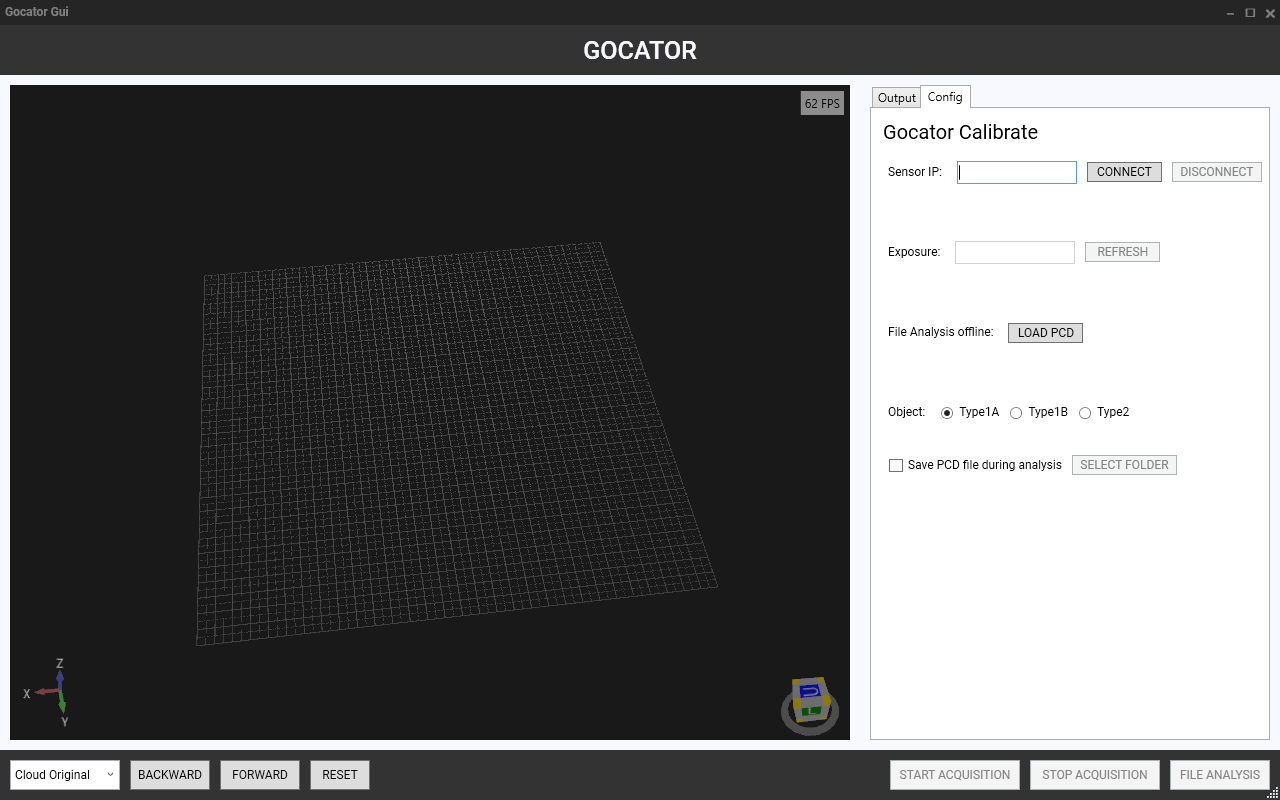
\includegraphics[width=1.0\columnwidth]{./pictures/gui_1.png}
	\caption{Interfaccia grafica con la descrizione dei pulsanti.}\label{fig:gui_1}
\end{figure}

\noindent Di seguito la descrizione dei pulsanti:

\begin{itemize}
	\item \textbf{1:} Connette e disconnette il sensore, tramite indirizzo IP;
	\item \textbf{2:} Aggiorna il valore dell'esposizione;
	\item \textbf{3:} Carica il file in formato \textit{.pcd} della \textit{point cloud} del battistrada;
	\item \textbf{4:} Seleziona il tipo di battistrada da analizzare;
	\item \textbf{5:} Seleziona la cartella dove salvare le \textit{point cloud}, create durante l'analisi;
	\item \textbf{6:} Visualizzatore 3D delle \textit{point cloud};
	\item \textbf{7:} Seleziona le \textit{point cloud} da visualizzare per oggetto scansionato;
	\item \textbf{8:} Scorre indietro le \textit{point cloud};
	\item \textbf{9:} Scorre avanti le \textit{point cloud};
	\item \textbf{10:} Resetta la visualizzazione e rimuove le \textit{point cloud} caricate;
	\item \textbf{11:} Avvia l'acquisizione dal Gocator;
	\item \textbf{12:} Interrompe l'acquisizione dal Gocator;
	\item \textbf{13:} Avvia l'analisi offline del file caricato;
\end{itemize}

\noindent Quindi, il programma può essere utilizzato sia in modalità online (connesso direttamente al Gocator) sia in modalità offline (caricando e analizzando il file della \textit{point cloud} del battistrada).\\
\newline
La modalità online permette di:

\begin{itemize}
	\item Inserire l'indirizzo IP del sensore, connettersi e disconnettersi;
	\item Modificare il valore dell'esposizione;
	\item Selezionare il tipo di battistrada da analizzare;
	\item Salvare i file in formato \textit{.pcd}, durante l'analisi, delle \textit{point cloud} step by step;
	\item Avviare e stoppare la scansione, con la visualizzazione del risultato dell'analisi in real time;
	\item Visualizzare a video le \textit{point cloud} dei battistrada scansionati e analizzati;
\end{itemize}

\noindent La modalità offline permette di:

\begin{itemize}
	\item Caricare un file contenente la \textit{point cloud} del battistrada;
	\item Selezionare il tipo di battistrada da analizzare;
	\item Salvare, durante l'analisi, le \textit{point cloud} step by step;
	\item Avviare l'analisi del file;
	\item Visualizzare a video le \textit{point cloud} caricate;
\end{itemize}

\begin{figure}[H]
	\centering
	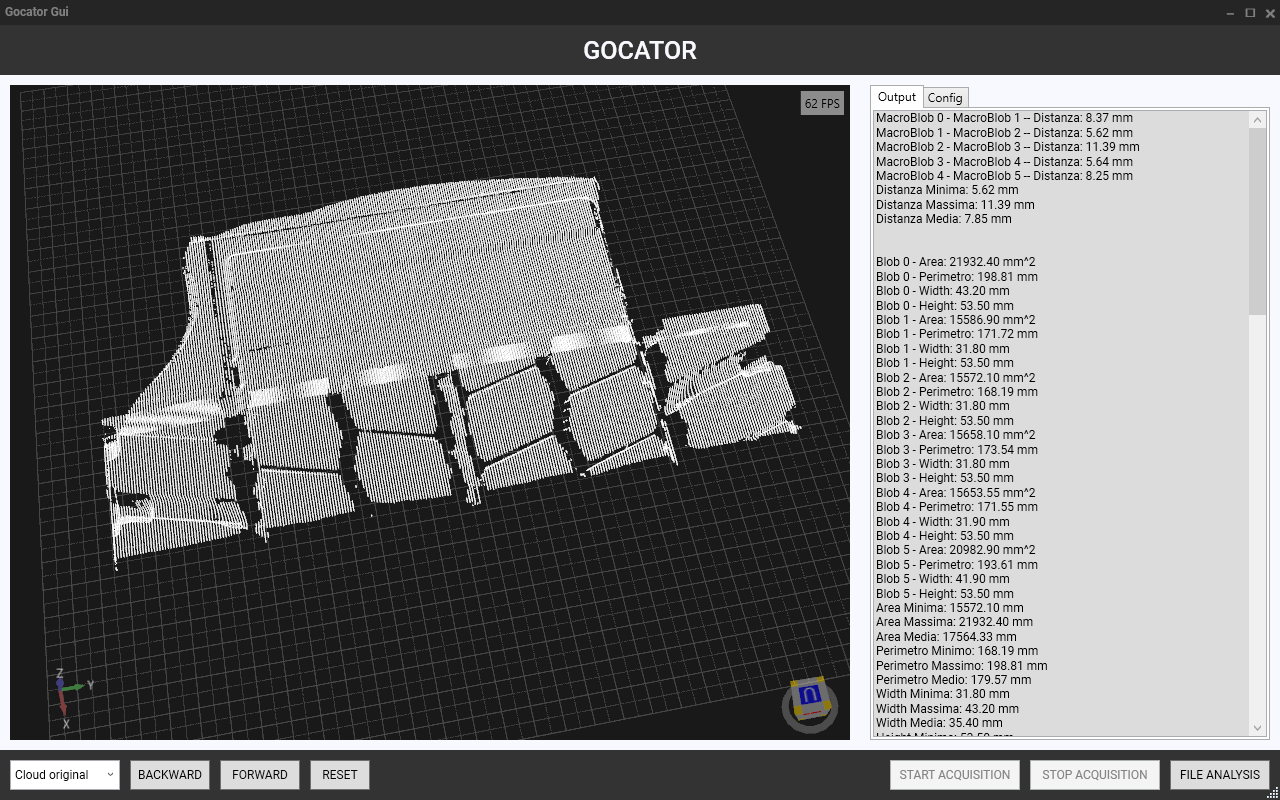
\includegraphics[width=0.9\columnwidth]{./pictures/gui_3.png}
	\caption{Interfaccia grafica con la point cloud filtrata visualizzata a video.}\label{fig:gui_2}
\end{figure}

\noindent In particolare, nel caso del battistrada di tipo \textit{2}, il risultato della scansione riporta a video, oltre alla \textit{point cloud} del battistrada, anche la stessa con evidenziati i punti di altezza delle scanalature minima e massima, e la \textit{point cloud} con solo i punti di massimo da sinistra e destra (figura \ref{fig:gui_4}, figura \ref{fig:gui_5} e figura \ref{fig:gui_6}).

\begin{figure}[H]
	\centering
	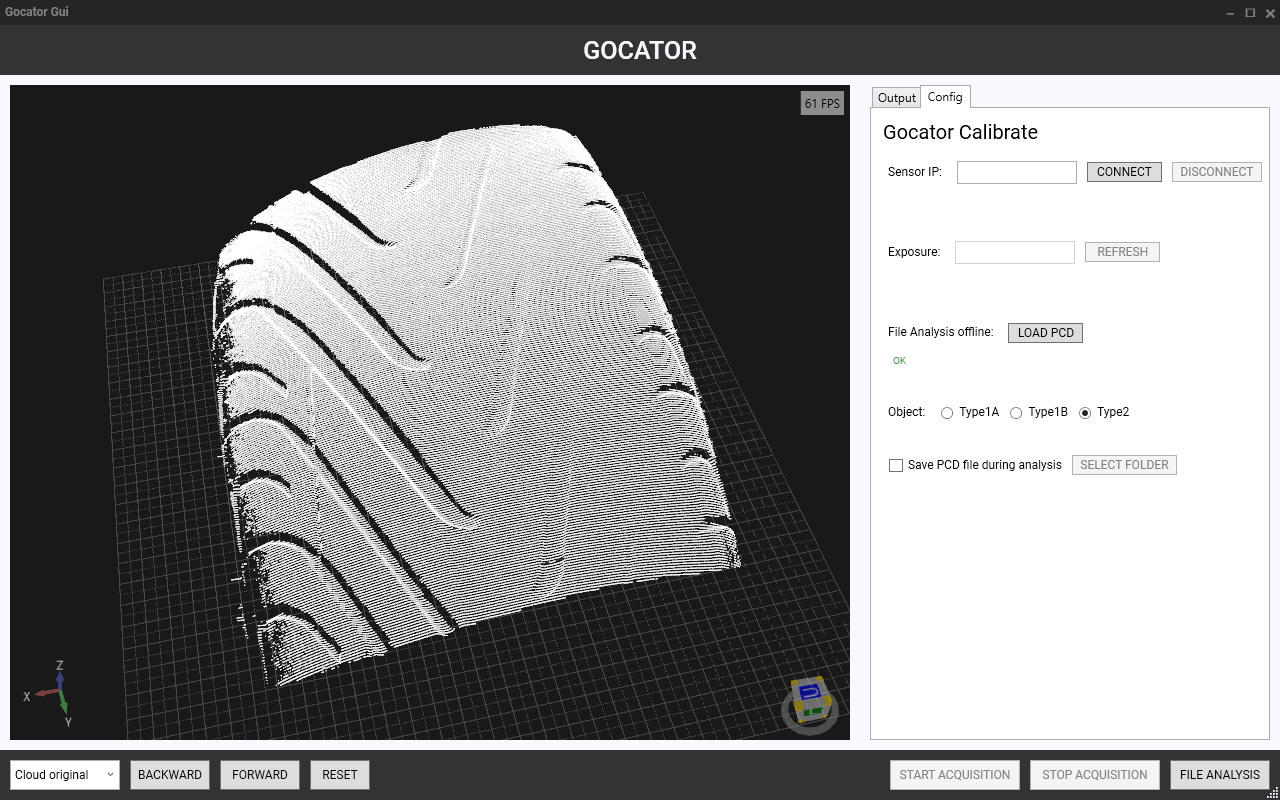
\includegraphics[width=0.9\columnwidth]{./pictures/gui_4.png}
	\caption{Interfaccia grafica con, visualizzata a video, la point cloud del battistrada di tipo 1A e il risultato dell'analisi.}\label{fig:gui_3}
\end{figure}

\begin{figure}[H]
	\centering
	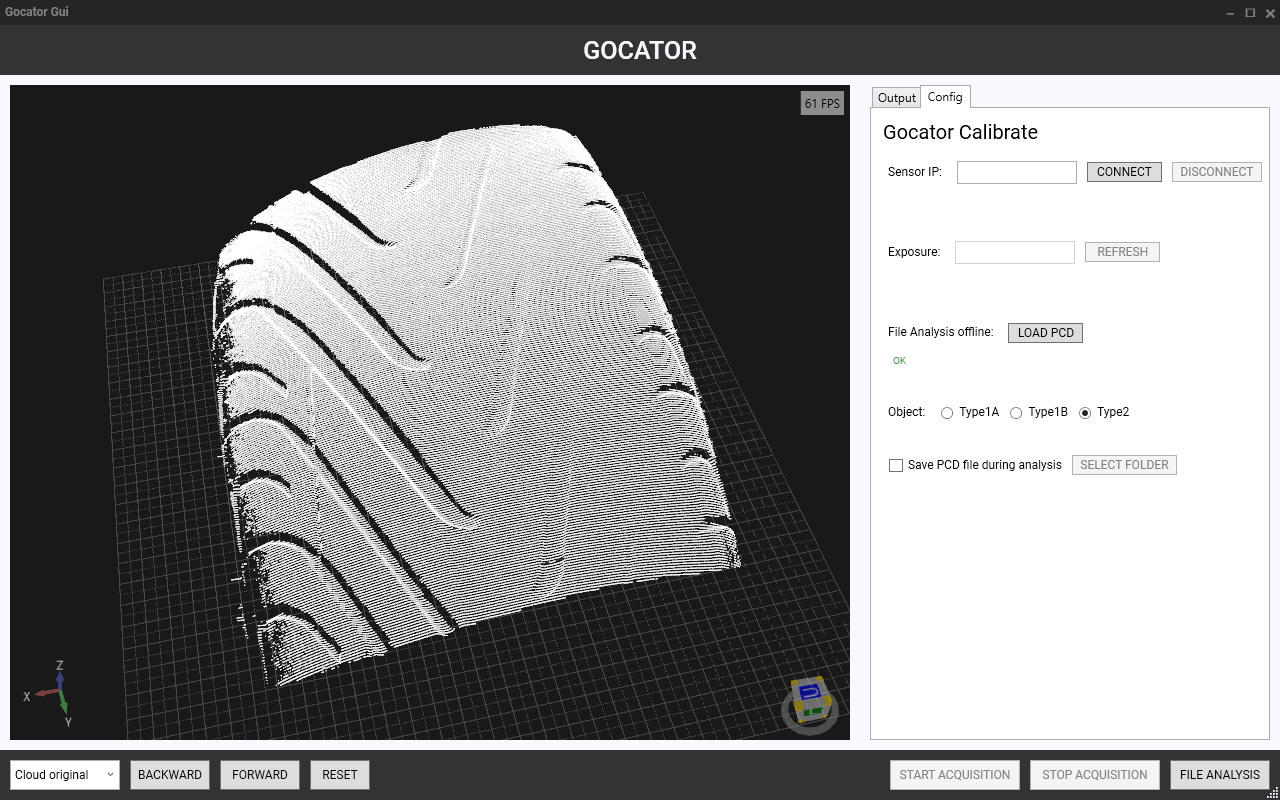
\includegraphics[width=0.9\columnwidth]{./pictures/gui_5.png}
	\caption{Interfaccia grafica con, visualizzata a video, la point cloud del battistrada di tipo 2.}\label{fig:gui_4}
\end{figure}

\begin{figure}[H]
	\centering
	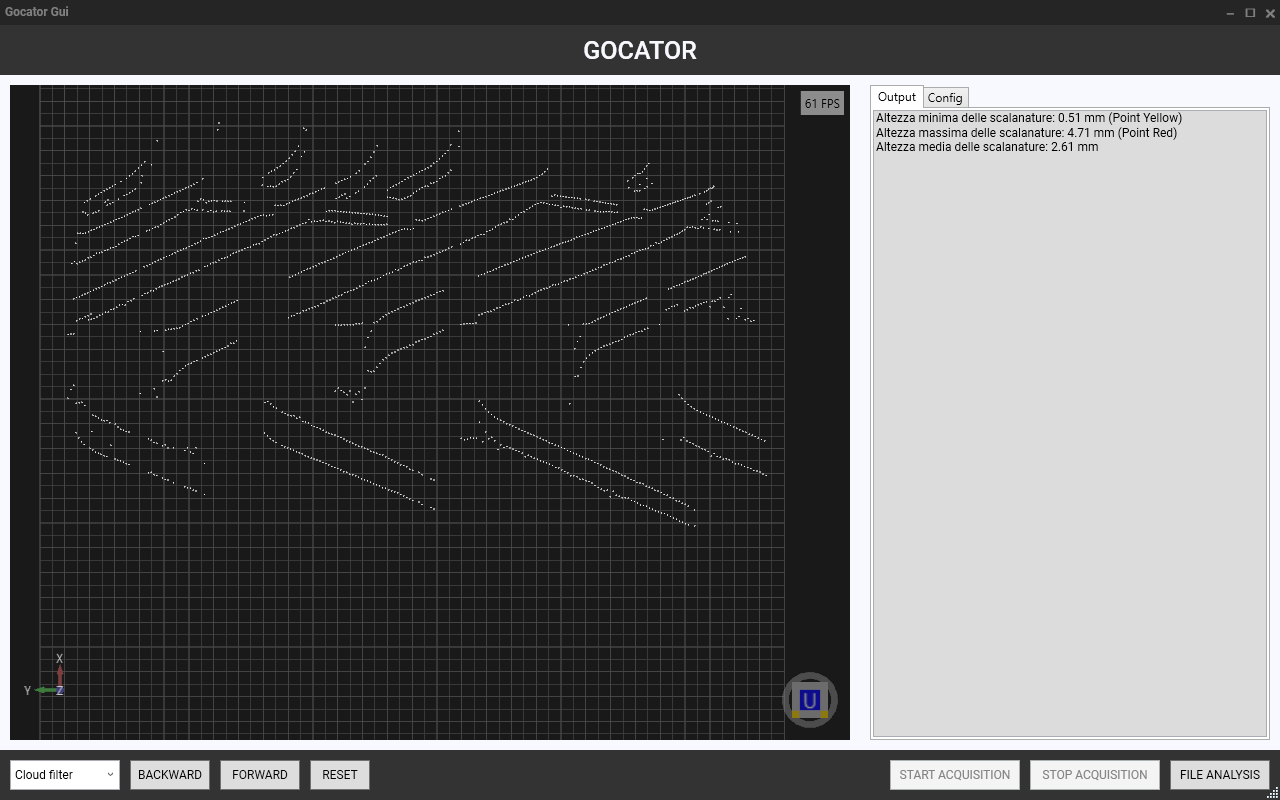
\includegraphics[width=0.9\columnwidth]{./pictures/gui_6.png}
	\caption{Interfaccia grafica con, visualizzata a video, la point cloud con i punti di profondità delle scanalature minima e massima.}\label{fig:gui_5}
\end{figure}

\begin{figure}[H]
	\centering
	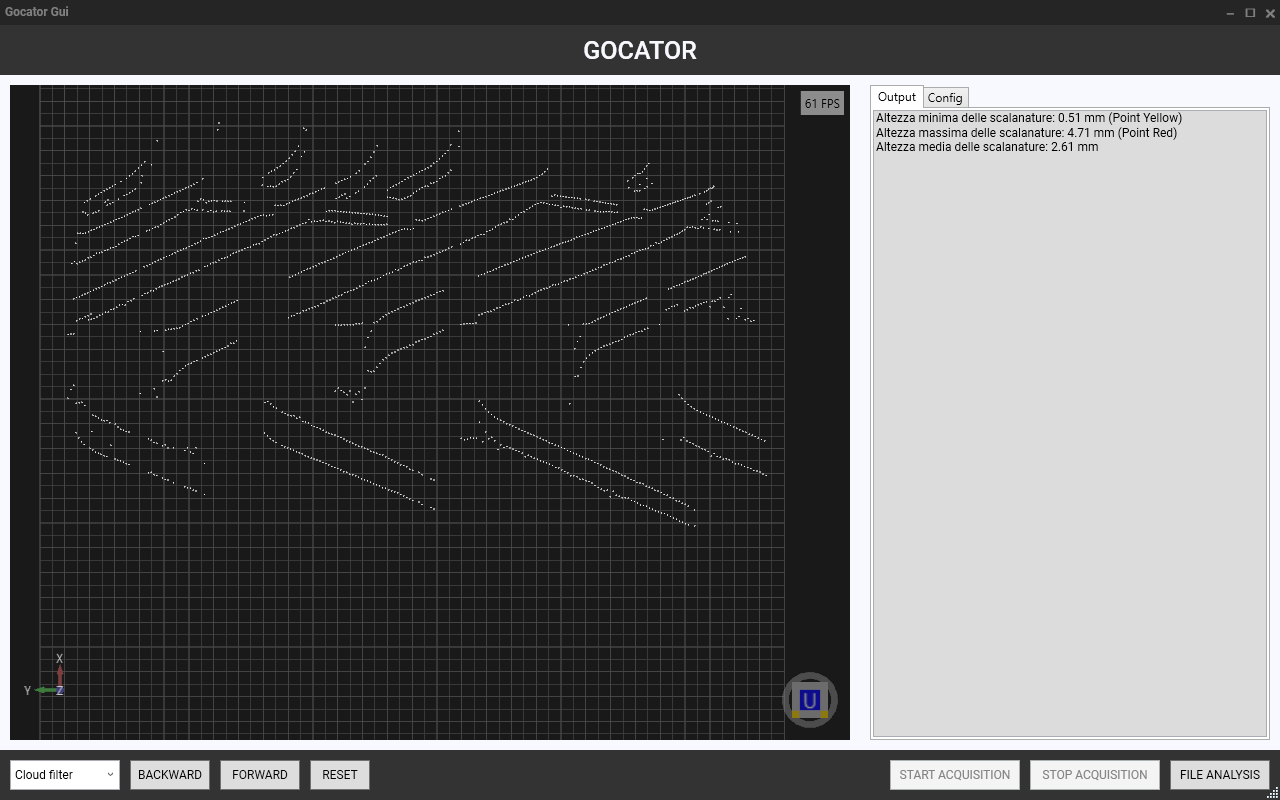
\includegraphics[width=0.9\columnwidth]{./pictures/gui_7.png}
	\caption{Interfaccia grafica con, visualizzata a video, la point cloud filtrata.}\label{fig:gui_6}
\end{figure}